\documentclass{article}
\usepackage{graphicx} % Required for inserting images
\usepackage[left=4cm, right=4cm, top=4cm, bottom=4cm]{geometry}
\usepackage[T1]{fontenc}
\usepackage[polish]{babel}
\usepackage{amssymb}
\usepackage{url}
\usepackage{enumitem}
\usepackage{dirtree}
\usepackage[export]{adjustbox}



\title{\Huge JIMP2 Projekt 2025 \\ {\huge Dokumentacja implementacyjna - C}}
\author{Michał Ludwiczak, Łukasz Leśniak \\ GR3}
\date{25 marca 2025}

\begin{document}

\maketitle

\tableofcontents



% Dokumentacja implementacyjna przedstawiająca szczegóły implementacyjne programu, specyfikacje wejścia oraz wyjścia, plików wyjściowych, etc.



\section{Cel projektu}

Celem projektu jest stworzenie aplikacji w języku C, dokonującej podziału grafu na określoną przez użytkownika lub domyślną liczbę 2 równych części z zachowaniem wybranego lub, ponownie, domyślnego 10-procentowego marginesu różnicy. Liczba wierzchołków w powstałych częściach grafu nie powinna się różnić o więcej niż zadany margines procentowy, a liczba przeciętych krawędzi pomiędzy wynikowymi częściami grafu powinna być jak najmniejsza. Wyjściem programu ma być plik tekstowy lub binarny. Użytkownik ma mieć możliwość wskazać wyjście programu, a więc plik tekstowy lub binarny, zawierający wynik działania programu, oraz dane wejściowe, które mogą być wykorzystane ponownie w kolejnym działaniu programu.



% wizualizacja problemu
\begin{figure}[ht]
    \centering
    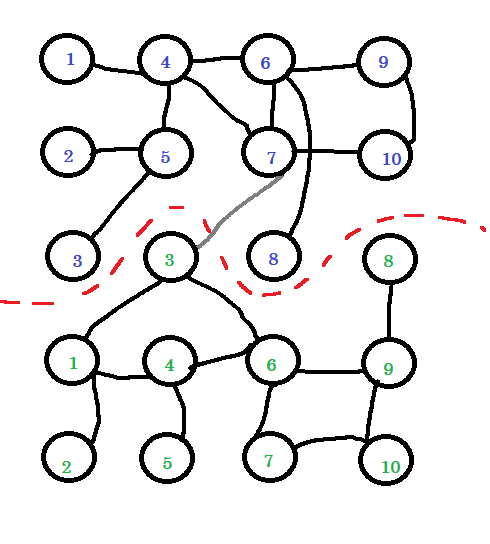
\includegraphics[width=0.75\linewidth]{img/graph.png}
    \caption{Przykładowy graf podzielony na 2 równe części}
    \label{fig:graph}
\end{figure}



\section{Algorytm}

Niestety znalezienie optymalnego podziału grafu należy do klasy problemów NP-trudnych. Dla grafu o \( n \) wierzchołkach istnieje aż \( 2^{n-1} - 1 \) możliwych sposobów na bisekcję (wyraźnego podziału na 2 grafy). \cite{youtube_video} Przy tego typu problemie nie możemy po prostu sprawdzić wszystkich możliwości i wybrać najlepszej z nich - jest to problem optymalizacji kombinatorycznej. W związku z tym opracowano wiele algorytmów zachłannych, metod przybliżonych i heurystyk, które pozwalają na uzyskanie satysfakcjonujących rozwiązań w praktyce.
W naszym programie zdecydowaliśmy się użyć algorytmu spektralnego, który wykorzystuje własności spektralne macierzy Laplace'a grafu. Na podstawie spektrum grafu, które opisuje strukturę jego strukturę, graf możemy podzielić w efektywny i satysfakcjonujący sposób, minimalizując liczbę przeciętych krawędzi.



    \subsection{Macierz Laplace'a}
    
    W podejściu spektralnym do podziału grafu kluczową rolę odgrywa macierz Laplace'a \cite{laplacian_matrix}.
    Wzór na Laplacian klasyczny definiuje się jako:
    \[
    \mathbf{L} = \mathbf{D} - \mathbf{A}
    \]
    gdzie:
    \begin{itemize}
      \item \( L \) to \textbf{macierz Laplace'a} grafu,
      \item \( D \) to \textbf{macierz stopni} to macierz diagonalna, w której elementy na diagonali \( d_{ii} \) odpowiadają stopniowi wierzchołka \( i \), czyli liczbie krawędzi, które są z nim bezpośrednio połączone (w przypadku pętli krawędź liczy się podwójnie)
      \item \( A \) to \textbf{macierz sąsiedztwa} grafu, gdzie elementy \( a_{ij} \) są równe 1, jeśli istnieje krawędź między wierzchołkami \( i \) i \( j \), oraz 0 w przeciwnym przypadku.
    \end{itemize}
    


    \subsection{Wektory własne}

    Następnym krokiem jest obliczenie \(k = p - 1\) (gdzie p to liczba części, na które graf ma być podzielony) najmniejszych wektorów własnych, nie wliczając pierwszego zerowego. Dla bisekcji będzie to tylko jeden wektor, drugi najmniejszy - wektor Fiedlera. Wektory własne macierzy Laplace'a grafu przechowują informacje o połączeniach pomiędzy wierzchołkami. 
    Istnieje metoda Lanczosa \cite{lanczos}, którą można zastosować na macierzy Laplace'a, gdyż jest to macierz symetryczna, a więc również i hermitowska. Generuje ona ortonormalną bazę przestrzeni Kryłowa oraz przekształca macierz Laplace'a do macierzy trójdiagonalnej \(T\). Z wartości i wektorów własnych tej uproszczonej macierzy i bazy Kryłowa można obliczyć przybliżenia wartości i wektorów własnych oryginalnej macierzy.

    
    
    \subsection{Klasteryzacja}

    Po otrzymaniu macierzy zawierającej wartości \(k\) wektorów własnych należy podzielić graf na \(p\) części. Te wartości są traktowane jako punkty w przestrzeni k-wymiarowej odpowiadające poszczególnym wierzchołkom. Stosuje się algorytm klasteryzacji, aby podzielić te wierzchołki na grupy, a tym samym podzielić graf na części. W naszym programie algorytmem klasteryzacji jest centroidów / k-średnich (k-means) \cite{k-means}. Wierzchołki w tych samych cześciach są ze sobą bardziej powiązane niż te, które są w innych częściach, co gwarantuje satysfakcjonujący podział.



    \subsection{Wynik}

    Po otrzymaniu poszczególnych części z wierzchołkami modyfikuje się macierz sąsiedztwa \(A\) wstawiając 0 w pola oznaczające krawędzie pomiędzy wierzchołkami przynależącymi do różnych grup. W ten sposób otrzymuje się nową macierz sąsiedztwa, która zawiera już podzielony graf. Macierz sąsiedztwa jest już gotowa do przetworzenia i wypisania na plik wyjściowy.
    



% Lista dostępnych flag sterujących programem, wraz z dokładnym opisem dopuszczalnych wartości argumentów tych flag
\section{Flagi i argumenty}

Program jest uruchamiany z linii poleceń i obsługuje następujące flagi:

\begin{description}
    \item[<plik\_wejściowy>] \hfill \\
    \textbf{input} \\
    Ścieżka do pliku wejściowego zawierającego opis grafu. \\
    \textit{Wymagane jako pierwszy argument}
    
    \item[-p \texttt{<liczba\_części>}] \hfill \\
    \textbf{parts} \\
    Określa liczbę części, na które ma zostać podzielony graf. \\
    \textit{Domyślnie:} 2
    
    \item[-m \texttt{<margines>}] \hfill \\
    \textbf{margin} \\
    Określa dopuszczalny margines procentowy różnicy w liczbie wierzchołków między częściami. \\
    \textit{Domyślnie:} 10\%
    
    \item[-o \texttt{<plik\_wyjściowy>}] \hfill \\
    \textbf{output} \\
    Określa ścieżkę do pliku wyjściowego, w którym zostaną zapisane wyniki. \\
    \textit{Domyślnie:} output.txt lub output.bin (w zależności od formatu)
    
    \item[-f \texttt{<format\_pliku\_wyjściowego>}] \hfill \\
    \textbf{format} \\
    Określa format pliku wyjściowego: \texttt{txt} dla pliku tekstowego lub \texttt{bin} dla pliku binarnego. \\
    \textit{Domyślnie:} txt
\end{description}



\section{Szczegóły implementacyjne}



    \subsection{Struktura plików}

    W projekcie obowiązuje poniższa struktura plików: \\

    \dirtree{%
    .1 JIMP2-Projekt-2025-C/.
    .2 src/.
    .2 include/.
    .2 input/.
    .2 output/.
    .2 docs/.
    .2 obj/.
    .2 Makefile.
    .2 .gitignore.
    } 

    \begin{itemize}
        \item \texttt{src/} \\
        Przechowywanie plików źródłowych (.c).
        \item \texttt{include/} \\
        Przechowywanie plików nagłówkowych (.h).
        \item \texttt{input/} \\
        Przechowywanie plików wejściowych (.csrrg).
        \item \texttt{output/} \\
        Przechowywanie plików wyjściowych (.txt, .bin).
        \item \texttt{docs/} \\
        Przechowywanie dokumentacji.
        \item \texttt{obj/} \\
        Przechowywanie plików wynikowych kompilacji typu object (.o). Folder ten jest tworzony i kasowany przez Makefile.
        \item \texttt{Makefile} \\
        Organizacja kompilacji programu.
        \item \texttt{.gitignore} \\
        Przechowywanie listy wyjątków - plików/folderów, które git powinien zignorować.
    \end{itemize}
    
    
    \subsection{Moduły}

    
    
    \begin{itemize}
        \item \texttt{main.c — plik główny} \\
        Wywołanie modułów w odpowiedniej kolejności. \\
        Parsowanie argumentów, wczytanie grafu z pliku wejściowego, utworzenie macierzy sąsiedzywa i macierzy Laplace'a, obliczenie wektorów własnych, klasteryzacja i podział grafu, wypisanie wyniku do pliku wyjściowego.
        Parsowanie argumentów, Wczytanie grafu, Przeprowadzenie podziału, Zapis wyniku.
        \item \texttt{config.h / config.c} \\
        Obsługa argumentów.
        \item \texttt{input.h / input.c} \\
        Wczytywanie grafu z pliku, reprezentacja grafu - macierz sąsiedztwa.
        \item \texttt{mat\_vec.h / mat\_vec.c} \\
        Odpowiedzialny za wektory, macierze oraz operacje na nich, w tym za utworzenie macierzy Laplace'a.
        \item \texttt{eigenvalues.h / eigenvalues.c} \\
        Implementacja algorytmu Lanczosa i obliczanie wartości wektorów własnych macierzy Laplace'a.
        \item \texttt{clusterization.h / clusterization.c} \\
        Implementacja algorytmu k-means do podziału grafu. Podział grafu.
        \item \texttt{output.h / output.c} \\
        Zapisanie wyniku w pliku wyjściowym w odpowiednim formacie.
    \end{itemize}



    \subsection{Struktury}
    
    \begin{itemize}
    
        \item \texttt{Config} \\
        Przechowywanie informacji podanych przez użytkownika wsadowo.
    
        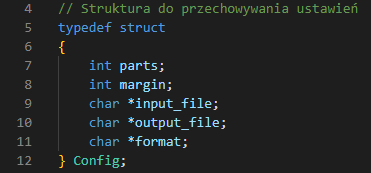
\includegraphics[width=0.65\linewidth, center]{img/config.png}
    
        \item \texttt{Input} \\
        Przechowywanie informacji pobranych z pliku wejściowego. Informacje te są później wykorzystywane m.in. do utworzenia macierzy sąsiedztwa.
    
        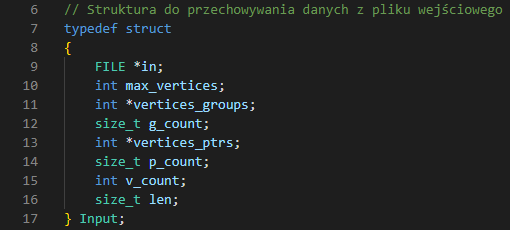
\includegraphics[width=0.75\linewidth, center]{img/input.png}

        \item \texttt{LanczosEigenV} \\
        Przechowywanie zmiennych do metody Lanczosa oraz do obliczania wartości własnych i przybliżonych wektorów własnych macierzy Laplace'a grafu.
    
        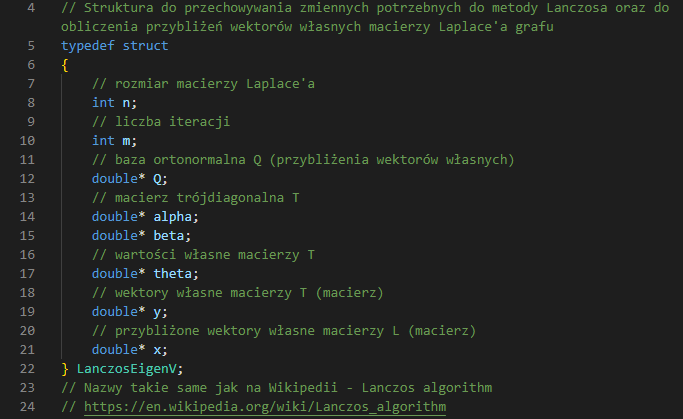
\includegraphics[width=0.825\linewidth, center]{img/lanczoseigenv.png}
    
    \end{itemize}

    
    
    \subsection{Najważniejsze funkcje}
    
    \begin{itemize}
    
        \item \texttt{parse\_args} \\
        Obsługa argumentów. Zapisanie konfiguracji do obiektu struktury Config. \\\\      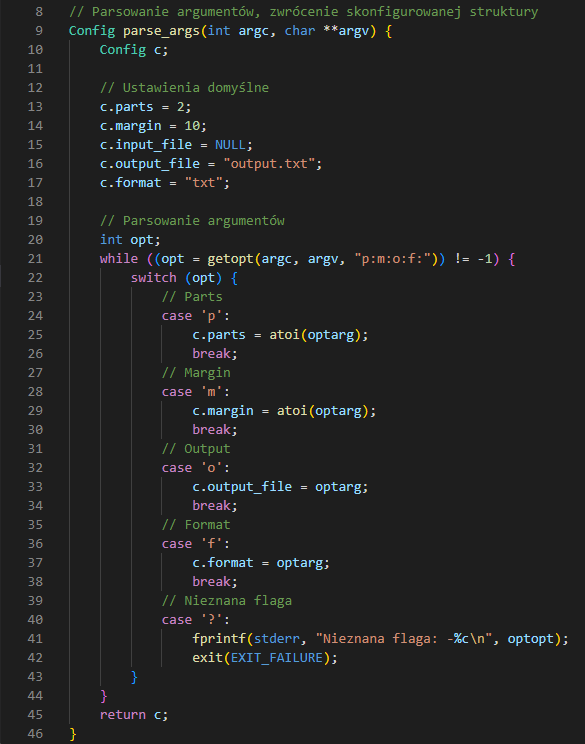
\includegraphics[width=0.825\linewidth, center]{img/parse_args.png}

        \item \texttt{read\_input} \\
        Wczytanie danych z pliku wejściowego do obiektu struktury Input. \\\\      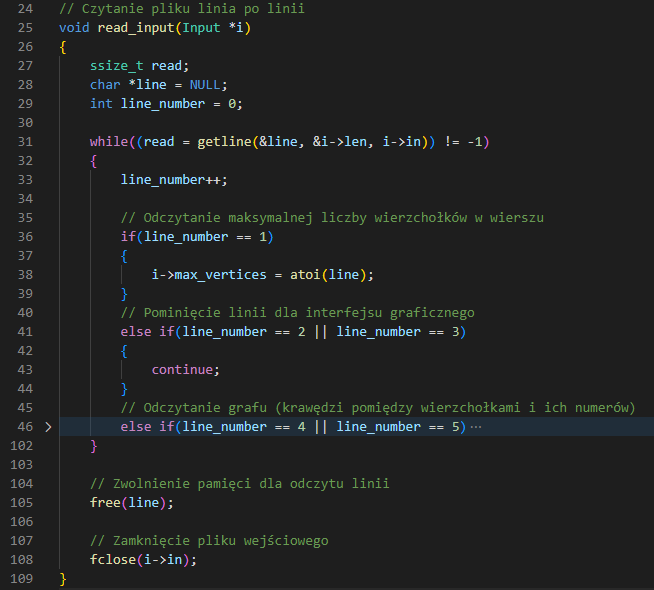
\includegraphics[width=0.825\linewidth, center]{img/read_input.png}
        
        \item \texttt{get\_adjacency\_matrix} \\
        Zapisanie grafu w formie macierzy sąsiedzywa. \\\\      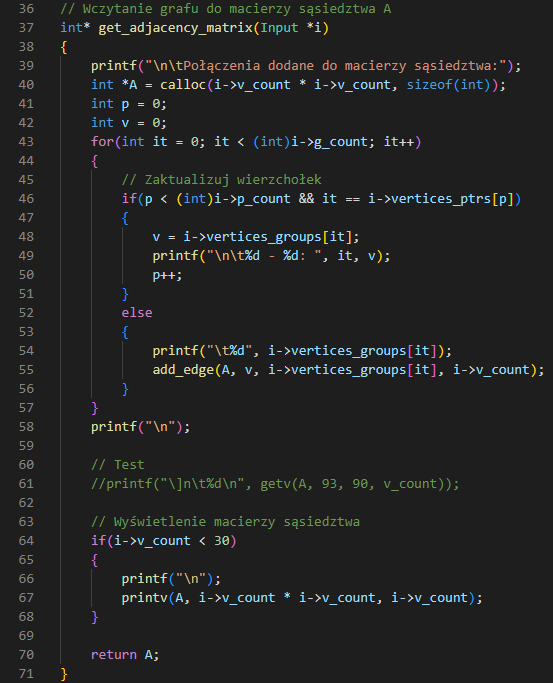
\includegraphics[width=0.825\linewidth, center]{img/get_adjacency_matrix.png}
        
        \item \texttt{calc\_laplacian} \\
        Obliczenie macierzy Laplace'a grafu. \\\\
        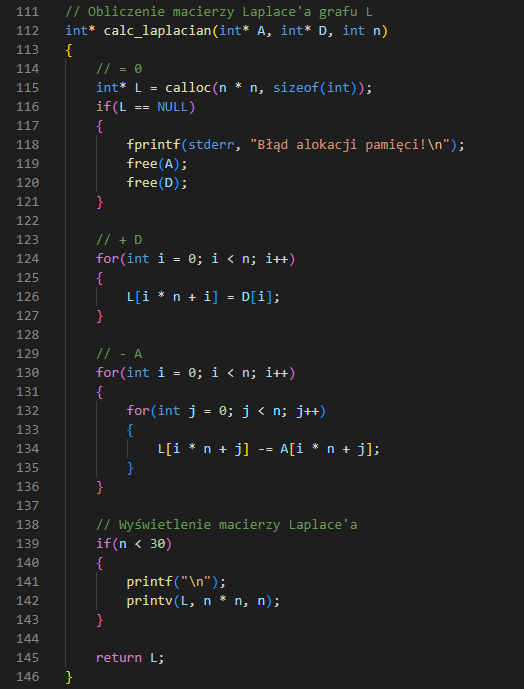
\includegraphics[width=0.825\linewidth, center]{img/calc_laplacian.png}
        
        \item \texttt{lanczos} \\
        Algorytm Lanczosa - obliczenie \(k\) wektorów własnych i zapisanie ich do macierzy. \\\\
        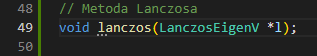
\includegraphics[width=0.825\linewidth, center]{img/lanczos.png}
        
        \item \texttt{clusterization} \\
        Algorytm klasteryzacji k-means (k-średnich) - podział wierzchołków na grupy. \\\\
        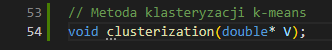
\includegraphics[width=0.825\linewidth, center]{img/clusterization.png}
        
        \item \texttt{write\_output} \\
        Wypisanie pliku wyjściowego z wynikiem i grafem. \\\\
        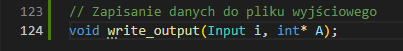
\includegraphics[width=0.825\linewidth, center]{img/write_output.png}
        
    \end{itemize}
    
    
    
    \subsection{Pliki wejściowe i wyjściowe}
    
    \begin{itemize}
    
        \item \textbf{Format plików wejściowych} \\
        Program akceptuje pliki wejściowe z rozszerzeniem .csrrg. Format danych wejściowych jest zdefiniowany za pomocą 5 linijek, z których każda odpowiada za zapis informacji.
        \begin{enumerate}[label=\arabic*.] % Użycie pakietu enumitem do numerowania
            \item Maksymalna możliwa liczba węzłów w wierszu (w grafie mogą być wiersze o ich mniejszej liczbie, ale nie o większej).
            \item Indeksy węzłów w poszczególnych wierszach – liczba wszystkich indeksów odpowiada liczbie węzłów grafu.
            \item Wskaźniki na pierwsze indeksy węzłów w liście wierszy z poprzedniego punktu.
            \item Grupy węzłów połączone przy pomocy krawędzi.
            \item Wskaźniki na pierwsze węzły w poszczególnych grupach z poprzedniego punktu. Ta sekcja może występować w pliku wielokrotnie, co oznacza, że plik zawiera więcej niż jeden graf.
        \end{enumerate}
        \textbf{Przykład:}
            \begin{center}
            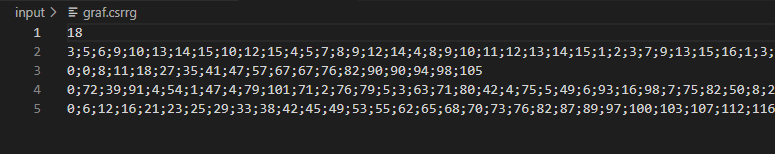
\includegraphics[width=1\linewidth]{img/grafcsrrg.png}
        \end{center}
    
        \item \textbf{Format plików wyjściowych} \\
    Pierwsza linijka pliku wyjściowego zawiera wynik działania programu w postaci: \\\\
    \texttt{<wynik (S - pomyślnie, F - nieudanie)> <liczba\_części> <zachowany\_margines>} \\\\
    Przykład: \texttt{S 2 0.045} \\\\
    Kolejne linijki są w takim samym formacie jak plik wejściowy i zawierają podział grafu. \\
    Wersja binarna zawiera te same informacje co tekstowa, ale w formie binarnej (struktury danych zapisane za pomocą \texttt{fwrite}).


        
    
    \end{itemize}



\begin{thebibliography}{9}

\bibitem{youtube_video}
Leonid Zhukov, \textit{Lecture 7. Graph partitioning algorithms.}, YouTube, 24 luty 2021, Dostępny na 1 kwietnia 2025 w: \url{https://youtu.be/zZae_C2BU_4}

\bibitem{laplacian_matrix}
\textit{Laplacian matrix}, Wikipedia, Dostępne na 1 kwietnia 2025 w: \url{https://en.wikipedia.org/wiki/Laplacian_matrix}

\bibitem{lanczos}
\textit{Lanczos algorithm}, Wikipedia, Dostępne na 1 kwietnia 2025 w:
\url{https://en.wikipedia.org/wiki/Lanczos_algorithm}

\bibitem{k-means}
\textit{Algorytm centroidów}, Wikipedia, Dostępne na 1 kwietnia 2025 w:
\url{https://pl.wikipedia.org/wiki/Algorytm_centroid%C3%B3w}

\end{thebibliography}



\end{document}
